\documentclass[11pt]{article}
\usepackage[review]{acl}
\usepackage{times}
\usepackage{latexsym}
\usepackage[T1]{fontenc}
\usepackage[utf8]{inputenc}
\usepackage{microtype}
\usepackage{inconsolata}
\usepackage{graphicx}
\usepackage{booktabs}
\usepackage{amsmath}
\usepackage[indonesian]{babel}
\usepackage{xurl}

\title{StereoQueerEval: Klasifikasi Ujaran Kebencian terhadap\
Komunitas LGBTQIA+ dengan XLM-RoBERTa dan Qwen3.5-9B}
% Identitas dan afiliasi diisi sebelum beralih ke mode final.
\author{Penulis Anonim}

\begin{document}
% Nomor halaman dipertahankan; nomor baris review dinonaktifkan.
\nolinenumbers
\raggedbottom
\maketitle
\begin{abstract}
% Evidence: Q001,Q002,Q004,Q005,B002.
Penelitian ini menyajikan pendekatan untuk menyelesaikan Subtask B SemEval-2027 Task 8: StereoQueerEval, yaitu mengklasifikasikan komentar YouTube ke dalam kelas \texttt{no}, \texttt{yes\_implicit}, dan \texttt{yes\_explicit}. XLM-RoBERTa Base digunakan sebagai pembanding, sedangkan pendekatan utama menyesuaikan Qwen3.5-9B menggunakan Low-Rank Adaptation (LoRA). Komentar dipertahankan dalam bahasa aslinya dan diproses tanpa judul serta deskripsi video. Qwen setelah pelatihan berlabel dievaluasi menggunakan prompt Inggris, Italia, dan Belanda. Seluruh pilihan prompt Qwen menghasilkan macro-F1 lebih tinggi daripada XLM-RoBERTa pada pengujian internal yang sama. Nilai macro-F1 tertinggi yang teramati adalah 0,719146 untuk Inggris, 0,7036 untuk Italia, dan 0,641522 untuk Belanda. Pada hasil per kelas yang tersedia, \texttt{no} memperoleh F1 tertinggi dan \texttt{yes\_implicit} memperoleh F1 terendah dalam setiap pasangan bahasa data dan prompt. Kesamaan bahasa prompt dan komentar belum menghasilkan skor tertinggi secara konsisten. Hasil ini berasal dari pengujian internal dan belum merupakan hasil evaluasi resmi shared task.
\end{abstract}

\section{Pendahuluan}
\label{sec:pendahuluan}
% Evidence: L102.
Deteksi ujaran kebencian tidak hanya berkaitan dengan pengenalan kata-kata kasar. Pesan yang menyerang kelompok tertentu juga dapat disampaikan melalui ungkapan tersirat yang membutuhkan pemahaman konteks. \citet{elsherief-etal-2021-latent} menjelaskan bahwa bahasa berkode dan ungkapan tidak langsung menjadi tantangan dalam mendeteksi ujaran kebencian yang disampaikan secara tidak langsung. Perbedaan cara penyampaian tersebut membuat model perlu mengenali maksud pesan, bukan hanya kata-kata yang muncul di dalamnya.

% Evidence: L111.
\citet{chan-etal-2024-hate} mengkaji deteksi ujaran kebencian terhadap komunitas LGBTQIA+ menggunakan GPT-3.5-turbo pada teks asli dan teks yang diterjemahkan ke bahasa Inggris. Penerjemahan memberikan hasil yang beragam; sebagian istilah slang dan ungkapan yang berkaitan dengan budaya tertentu tidak diterjemahkan dengan tepat. Temuan tersebut menjadi pertimbangan untuk mempertahankan bahasa asli komentar. Penelitian itu juga menyarankan penggunaan prompt dalam bahasa data serta pengujian model lain. Saran tersebut menjadi salah satu dasar penyusunan prompt klasifikasi dalam penelitian ini.

% Evidence: L110,L117,Q001,B002.
Penelitian ini berfokus pada penyelesaian \textit{Subtask B: Hate Speech Classification} dalam SemEval-2027 Task 8: StereoQueerEval. Teks yang diklasifikasikan berupa komentar berbahasa Inggris, Italia, dan Belanda. Setiap komentar diberi label \texttt{no}, \texttt{yes\_implicit}, atau \texttt{yes\_explicit}. XLM-RoBERTa Base digunakan sebagai pembanding, sedangkan pendekatan utama menggunakan Qwen3.5-9B yang disesuaikan dengan data task. Keduanya dinilai pada komentar uji yang sama.

% Evidence: Q001,Q002,Q004,Q006,B002.
Penyelesaian task dilakukan melalui penyiapan data, pelatihan model, dan penentuan satu label untuk setiap komentar. Pada Qwen, definisi kategori diberikan melalui prompt berbahasa Inggris, Italia, atau Belanda. Ketiga pilihan digunakan untuk menemukan pengaturan yang sesuai bagi klasifikasi, dengan tetap mempertahankan bahasa asli komentar. Hasil evaluasi dilaporkan sebagai macro-F1 pada setiap bahasa data dan F1 setiap kelas, sesuai nilai yang tersedia dalam ringkasan eksperimen.

\section{Deskripsi Task}
\subsection{SemEval-2027 Task 8: StereoQueerEval}
\label{sec:task}
% Evidence: L110,L117.
StereoQueerEval merupakan task identifikasi stereotip dan ujaran kebencian yang menargetkan komunitas LGBTQIA+.\footnote{\url{https://semeval.github.io/SemEval2027/tasks.html}} Data berupa komentar YouTube yang disertai judul dan deskripsi video sebagai informasi konteks. Task ini terdiri atas deteksi stereotip, klasifikasi ujaran kebencian, serta identifikasi target dan identitas LGBTQIA+ yang menjadi sasaran kebencian \citep{stereoqueereval-2026-data}.

Penelitian ini berfokus pada Subtask B. Setiap komentar diberi salah satu dari tiga label berikut:
\begin{itemize}
    \item \texttt{no}: komentar yang tidak mengandung ujaran kebencian, termasuk komentar yang mendukung komunitas LGBTQIA+.
    \item \texttt{yes\_implicit}: kebencian yang disampaikan secara tersirat atau tidak langsung.
    \item \texttt{yes\_explicit}: kebencian yang dinyatakan secara langsung terhadap individu atau kelompok LGBTQIA+.
\end{itemize}

% Evidence: L110,Q001,Q005.
Data StereoQueerEval tersedia dalam bahasa Inggris, Italia, Belanda, dan Persia. Percobaan ini menggunakan tiga bahasa pertama, yang selanjutnya disingkat EN, IT, dan NL. Masukan utama berupa teks komentar. Pada Qwen, penanda bahasa disertakan bersama komentar. Judul, deskripsi video, dan anotasi dari subtask lain tidak digunakan untuk menentukan label.

\subsection{Penelitian Terkait}
% Evidence: L101,L114,L112.
Deteksi kebencian terhadap komunitas LGBTQIA+ telah dikaji dengan model klasifikasi maupun model bahasa besar. \citet{nozza-2022-nozza} menggabungkan prediksi BERT, RoBERTa, dan HateBERT untuk mengenali homofobia dan transfobia pada komentar YouTube Inggris. QUEEREOTYPES menyediakan anotasi stereotip dan ujaran kebencian secara terpisah pada data Italia \citep{cignarella-etal-2024-queereotypes}. Sementara itu, \citet{nguyen-etal-2025-leveraging} mengevaluasi lima model bahasa besar untuk mengenali teks anti-LGBTQIA+ tanpa pelatihan tambahan dan melaporkan bahwa kesalahan klasifikasi masih terjadi.

% Evidence: L111,L115,L104.
\citet{chan-etal-2024-hate} membandingkan GPT-3.5-turbo sebelum dan sesudah pelatihan pada data berlabel. Hasilnya mendukung penggunaan pelatihan untuk klasifikasi multibahasa, tetapi tugasnya menggunakan dua kelas dan weighted-F1. Penelitian ini membedakan tiga kelas dan menggunakan macro-F1, sehingga nilai kedua penelitian tidak dibandingkan secara langsung. XLM-RoBERTa dipilih sebagai pembanding karena prapelatihannya menggunakan teks dari 100 bahasa \citep{conneau-etal-2020-unsupervised}, sedangkan LoRA memungkinkan penyesuaian Qwen melalui sejumlah kecil parameter tambahan \citep{hu-etal-2021-lora}.

% Evidence: L116,Q001,Q006.
Pilihan bahasa prompt juga perlu diperhatikan ketika menggunakan model multibahasa. \citet{behzad-etal-2024-ask} menemukan bahwa prompt dalam bahasa berbeda dapat menghasilkan nilai yang berbeda pada penilaian tata bahasa Inggris. Temuan tersebut berasal dari tugas lain, sehingga menjadi pertimbangan untuk menguji pilihan prompt, bukan bukti langsung tentang deteksi kebencian. Dalam penyelesaian StereoQueerEval ini, tiga bahasa prompt digunakan pada tahap pelatihan dan pengujian Qwen.

\section{Metodologi}
\subsection{XLM-RoBERTa}
% Evidence: L115,B002.
XLM-RoBERTa merupakan model Transformer multibahasa yang dilatih menggunakan lebih dari 2 TB teks CommonCrawl dari 100 bahasa \citep{conneau-etal-2020-unsupervised}. Varian Base, selanjutnya disebut XLM-R, digunakan sebagai pembanding dalam penelitian ini. Teks komentar diubah menjadi token, kemudian diproses untuk memperoleh representasi yang mempertimbangkan hubungan antarkata. Representasi tersebut diteruskan ke lapisan klasifikasi untuk memprediksi tiga kelas task.

Seluruh parameter XLM-RoBERTa dan lapisan klasifikasi diperbarui menggunakan data pelatihan. Pelatihan menggunakan bobot kelas yang dihitung dari jumlah contoh pada data pelatihan agar kelas yang lebih sedikit mendapat perhatian dalam perhitungan kesalahan. Model dengan macro-F1 validasi tertinggi digunakan untuk pengujian.

\subsection{Qwen3.5-9B}
% Evidence: Q001,Q004,L103,L104.
Qwen3.5-9B digunakan sebagai model bahasa yang menerima prompt klasifikasi \citep{qwen-team-2026-qwen35}. Model disesuaikan melalui \textit{supervised fine-tuning} (SFT), yaitu pelatihan menggunakan komentar dan jawaban yang benar. Penyesuaian dilakukan dengan LoRA, yang mempertahankan bobot utama model dan memperbarui parameter tambahan berukuran kecil \citep{hu-etal-2021-lora}.

% Evidence: Q001,Q004,Q006.
Prompt menjelaskan ketiga kategori dan menegaskan bahwa penyebutan identitas LGBTQIA+ saja tidak cukup untuk menganggap komentar sebagai kebencian. Prompt tersedia dalam bahasa Inggris, Italia, dan Belanda, tanpa contoh komentar berlabel. Jawaban yang diminta berupa satu angka: 0 untuk \texttt{no}, 1 untuk \texttt{yes\_explicit}, dan 2 untuk \texttt{yes\_implicit}. Teks komentar tetap menggunakan bahasa aslinya. Penanda bahasa dan komentar pada masukan tetap ditulis dalam bahasa Inggris untuk seluruh pilihan prompt.

% Evidence: Q001,Q004.
Pelatihan diarahkan pada jawaban yang benar, sedangkan prompt dan komentar tidak dimasukkan ke perhitungan kesalahan pelatihan. Saat prediksi, model menghitung jumlah log probabilitas setiap pilihan jawaban beserta penanda akhirnya. Jawaban dengan skor tertinggi menjadi label prediksi. Dengan aturan ini, hasil selalu berupa salah satu dari tiga kategori dan tidak bergantung pada penjelasan bebas dari model.

\subsection{Alur Analisis}
% Evidence: Q001,Q004,Q005,Q006,B002.
Alur analisis meliputi eksplorasi data, prapemrosesan dan pembagian data, pelatihan dan prediksi, serta evaluasi model. XLM-RoBERTa mempelajari klasifikasi langsung dari teks komentar, sedangkan Qwen menerima definisi kategori dan komentar dalam format percakapan. Kedua pendekatan menghasilkan satu label untuk setiap komentar. Langkah analisis diterapkan pada setiap bahasa data secara terpisah.

\subsubsection{Eksplorasi Data (EDA)}
% Evidence: Q007.
Eksplorasi data atau exploratory data analysis (EDA) dilakukan pada dataset sebelum pembagian. Pemeriksaan meliputi jumlah komentar pada setiap bahasa dan kelas, kelengkapan kolom, keunikan ID, serta duplikasi komentar. Visualisasi distribusi kelas digunakan untuk memahami ketidakseimbangan label.

\subsubsection{Prapemrosesan dan Pembagian Data}
% Evidence: Q001,Q005,Q007,B002,L118.
Prapemrosesan menggunakan normalisasi Unicode NFKC untuk menyeragamkan representasi karakter yang setara \citep{unicode-consortium-2026-normalization}. Tujuannya mengurangi variasi penulisan Unicode agar kesamaan teks dapat diperiksa secara lebih konsisten. Kapitalisasi, emoji, dan tanda baca dipertahankan, serta komentar tidak diterjemahkan.

% Evidence: Q005,Q007.
Pembagian dilakukan terpisah untuk setiap bahasa dengan stratifikasi label, pengelompokan konteks video, dan seed 42. Target pembagiannya adalah 70\% pelatihan, 10\% validasi, dan 20\% pengujian. Komentar dengan pasangan judul--deskripsi yang sama atau komentar duplikat setelah normalisasi ditempatkan dalam kelompok yang sama. Kelompok tersebut dipertahankan pada satu bagian data agar tidak terpecah antara pelatihan, validasi, dan pengujian.

% Evidence: Q001,Q004,B002.
Setelah pembagian, komentar ditokenisasi menggunakan tokenizer masing-masing model dan dipotong jika melebihi batas masukan yang ditetapkan. Pada Qwen, ruang untuk prompt dan pilihan jawaban tetap disediakan. Prosedur pembagian yang sama digunakan untuk kedua model.

\subsubsection{Pelatihan dan Prediksi}
% Evidence: Q001,Q004,Q006,B002.
Data pelatihan digunakan untuk memperbarui parameter model. Setelah setiap epoch, hasil pada data validasi dihitung untuk memilih hasil pelatihan dengan macro-F1 tertinggi. Model terpilih kemudian memprediksi label komentar uji menggunakan aturan klasifikasi masing-masing model. Label yang benar pada data uji hanya digunakan untuk menghitung metrik evaluasi.

\subsubsection{Evaluasi Model}
% Evidence: Q001,Q003,Q004,Q005,B002.
Evaluasi dilakukan setelah model dipilih berdasarkan hasil validasi. Label prediksi dibandingkan dengan label yang benar pada komentar uji yang sama untuk kedua pendekatan. Hasil disajikan sebagai macro-F1 untuk setiap pasangan bahasa data dan prompt, serta F1 setiap kelas. Pengujian ini merupakan evaluasi internal karena komentar uji berasal dari pembagian data pelatihan penyelenggara, bukan dari data uji resmi shared task.

\subsection{Metrik Evaluasi}
% Evidence: Q001,Q002,Q003,Q004,B002.
Ukuran utama adalah macro-F1, yaitu rata-rata F1 dari tiga kelas dengan bobot yang sama. Precision menunjukkan proporsi prediksi suatu kelas yang benar, sedangkan recall menunjukkan proporsi contoh kelas tersebut yang berhasil dikenali. F1 menggabungkan precision dan recall sehingga dapat merangkum keduanya.

\section{Rancangan Eksperimen}
% Evidence: Q005,Q007,L110.
Dataset berasal dari komentar YouTube yang dirilis penyelenggara StereoQueerEval dan disertai informasi konteks video. Penelitian ini menggunakan total 7.627 komentar berlabel untuk klasifikasi tiga kelas. Teks komentar digunakan sebagai masukan utama, sedangkan judul dan deskripsi membantu pemeriksaan kelompok konteks saat pembagian. Pengujian dilakukan pada pembagian internal data pelatihan penyelenggara, bukan pada data uji resmi shared task.

\begin{table}[ht]
\centering
\small
\setlength{\tabcolsep}{3pt}
\begin{tabular}{llrrr}
\toprule
Bahasa & Kelas & Latih & Validasi & Uji \\
\midrule
EN & \texttt{no} & 983 & 147 & 277 \\
EN & \texttt{yes\_implicit} & 546 & 70 & 156 \\
EN & \texttt{yes\_explicit} & 582 & 75 & 153 \\
EN & Total & 2111 & 292 & 586 \\
IT & \texttt{no} & 822 & 105 & 233 \\
IT & \texttt{yes\_implicit} & 401 & 56 & 124 \\
IT & \texttt{yes\_explicit} & 476 & 59 & 124 \\
IT & Total & 1699 & 220 & 481 \\
NL & \texttt{no} & 784 & 109 & 234 \\
NL & \texttt{yes\_implicit} & 335 & 55 & 97 \\
NL & \texttt{yes\_explicit} & 437 & 62 & 125 \\
NL & Total & 1556 & 226 & 456 \\
\bottomrule

\end{tabular}
\caption{Jumlah komentar setiap kelas setelah pembagian. Latih, validasi, dan uji masing-masing berarti data pelatihan, validasi, dan pengujian.}
\label{tab:split}
\end{table}

% Evidence: Q005,Q007,B002.
Tabel~\ref{tab:split} memperlihatkan jumlah komentar setelah pembagian. Data pelatihan berjumlah 2.111 pada Inggris, 1.699 pada Italia, dan 1.556 pada Belanda. Data validasi masing-masing berjumlah 292, 220, dan 226, sedangkan data pengujian berjumlah 586, 481, dan 456. Ketiga kelas hadir pada seluruh bagian. Seluruh baris tetap teralokasi dengan isi komentar yang sama seperti sebelum pembagian. Pemeriksaan tidak menemukan overlap ID, komentar ternormalisasi, atau pasangan judul--deskripsi nonkosong antarbagian. Duplikasi komentar pada Italia berada dalam bagian pelatihan yang sama. Konteks judul--deskripsi tetap merupakan pendekatan untuk mengenali kelompok video, bukan jaminan identitas video yang sempurna.


% Evidence: Q001,Q002,Q004,Q006,B002.
Eksperimen membandingkan XLM-RoBERTa Base dengan Qwen3.5-9B yang disesuaikan menggunakan SFT LoRA. XLM-R dilatih satu kali untuk setiap bahasa, sedangkan Qwen dilatih untuk sembilan pasangan bahasa komentar dan bahasa prompt. Setiap pasangan Qwen dimulai dari model dasar yang sama dengan parameter LoRA baru. Prompt yang dipilih digunakan secara konsisten selama pelatihan, validasi, dan pengujian. Kedua model menggunakan pembagian data yang sama.

% Evidence: Q001,Q004,B002.
Pelatihan dan evaluasi model dilakukan menggunakan Python dan PyTorch dengan GPU melalui platform Modal.

% Evidence: Q001,Q004,B002,L109.
Kedua model menggunakan AdamW \citep{loshchilov-hutter-2019-decoupled}, seed 42, dan weight decay sebesar 0,01. XLM-R dilatih selama paling banyak 10 epoch dengan learning rate $10^{-5}$, batch pelatihan 32, dan batas masukan 384 token. Learning rate diturunkan secara linear tanpa tahap pemanasan.

% Evidence: Q001,Q004,Q008.
Qwen dilatih selama paling banyak lima epoch dengan learning rate $10^{-4}$ dan batas masukan 1.024 token. Setiap batch berisi empat komentar dengan akumulasi empat langkah, sehingga batch efektifnya adalah 16. LoRA menggunakan rank 16, alpha 32, dan dropout 0,05. Learning rate mengikuti penjadwalan cosine dengan tahap pemanasan sekitar 5\% dari rencana langkah pelatihan.

% Evidence: Q001,Q002,Q004,Q008,B002.
Evaluasi dilakukan pada akhir setiap epoch. Pelatihan dihentikan lebih awal jika macro-F1 validasi tidak membaik dalam tiga evaluasi untuk XLM-R atau dua evaluasi untuk Qwen. Model dengan macro-F1 validasi tertinggi dalam setiap percobaan digunakan untuk pengujian. Jika suatu pasangan diulang, hasil yang dilaporkan mengikuti percobaan terbaru yang dicatat dalam ringkasan eksperimen. Nilai pengujian tidak digunakan untuk memilih percobaan. Skor tertinggi pada tabel hasil disajikan secara deskriptif; pemilihan pengaturan untuk pengujian berikutnya perlu menggunakan data validasi.

\section{Hasil dan Pembahasan}
\subsection{Eksplorasi Data (EDA)}
% Evidence: Q007.
Dataset sebelum pembagian terdiri atas 2.989 komentar Inggris, 2.400 Italia, dan 2.238 Belanda. Gambar~\ref{fig:eda-labels} menunjukkan bahwa kelas \texttt{no} memiliki jumlah terbesar, yaitu 1.407 pada Inggris, 1.160 pada Italia, dan 1.127 pada Belanda. Jumlah \texttt{yes\_implicit} masing-masing adalah 772, 581, dan 487, sedangkan \texttt{yes\_explicit} berjumlah 810, 659, dan 624.

\begin{figure*}[t]
\centering
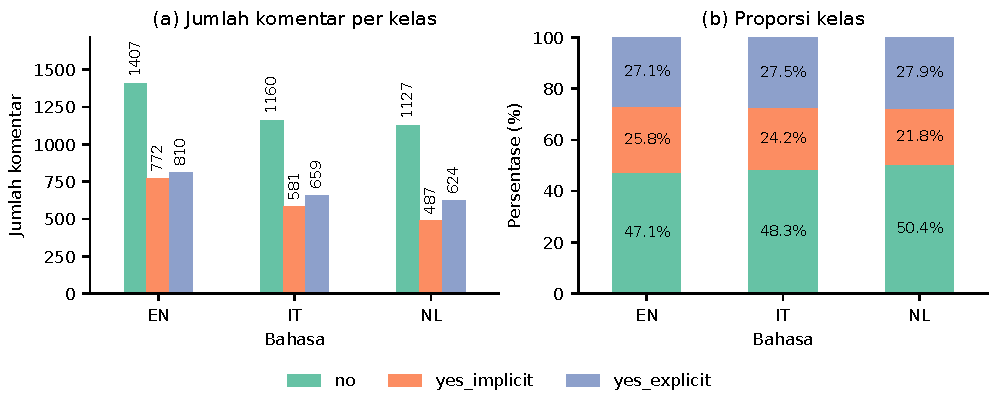
\includegraphics[width=\textwidth]{figures/eda_label_distribution.pdf}
\caption{Jumlah dan proporsi kelas sebelum pembagian, berdasarkan notebook EDA. Panel kiri menunjukkan jumlah komentar dan panel kanan menunjukkan persentase pada setiap bahasa.}
\label{fig:eda-labels}
\end{figure*}

% Evidence: Q007.
Kelas \texttt{no} menyumbang hampir separuh komentar pada ketiga bahasa. Proporsinya adalah 47,07\% pada Inggris, 48,33\% pada Italia, dan 50,36\% pada Belanda. Kelas terkecil adalah \nolinkurl{yes_implicit}, dengan proporsi masing-masing 25,83\%, 24,21\%, dan 21,76\%. Komposisi tersebut mendukung penggunaan macro-F1 agar setiap kelas mendapat bobot yang sama dalam evaluasi. Pada XLM-R, bobot kelas untuk pelatihan dihitung hanya dari data pelatihan masing-masing bahasa.

% Evidence: Q007.
Pemeriksaan tidak menemukan nilai kosong pada kolom identitas, komentar, konteks video, dan label yang dianalisis. Seluruh ID unik dan semua label sesuai tiga kelas task. Pada data Italia terdapat satu duplikasi komentar setelah normalisasi, tanpa perbedaan label.

\subsection{Hasil Klasifikasi}
% Evidence: Q002,B002.
Tabel~\ref{tab:main} membandingkan XLM-R yang dilatih per bahasa dengan Qwen setelah SFT pada sembilan pasangan bahasa data dan prompt. Pada data Inggris, hasil tertinggi diperoleh dengan prompt Inggris sebesar 0,719146. Pada Italia, prompt Inggris memperoleh skor tertinggi sebesar 0,7036, sedangkan pada Belanda skor tertinggi diperoleh dengan prompt Belanda sebesar 0,641522. Nilai tersebut menunjukkan hasil tertinggi yang teramati pada pengujian internal, bukan pengaturan akhir yang dipilih melalui data validasi.

\begin{table*}[t]
\centering
\small
\setlength{\tabcolsep}{3pt}
\begin{tabular}{lrrrr}
\toprule
Data & XLM-RoBERTa & Prompt EN & Prompt IT & Prompt NL \\
\midrule
EN & 0.529052 & \textbf{0.719146} & 0.715757 & 0.688340 \\
IT & 0.574515 & \textbf{0.7036} & 0.694249 & 0.701449 \\
NL & 0.507678 & 0.629927 & 0.630810 & \textbf{0.641522} \\
\bottomrule

\end{tabular}
\caption{Macro-F1 XLM-RoBERTa sebagai pembanding dan Qwen setelah SFT. Nilai Qwen mengikuti ringkasan eksperimen. Cetak tebal menunjukkan nilai Qwen tertinggi pada setiap bahasa data.}
\label{tab:main}
\end{table*}

% Evidence: B002,Q002.
Pada Inggris, XLM-R memperoleh macro-F1 sebesar 0,529052. Skor pada Italia dan Belanda masing-masing adalah 0,574515 dan 0,507678. Semua pilihan prompt Qwen menghasilkan skor lebih tinggi daripada pembanding tersebut. Hasil kedua pendekatan berasal dari komentar uji yang sama. Kedua model menggunakan teks komentar yang sama, tetapi ukuran model, tokenizer, batas masukan, dan cara pelatihannya berbeda. Oleh karena itu, selisih skor belum dapat dikaitkan dengan satu komponen tertentu.

\subsection{Analisis Berdasarkan Bahasa}
% Evidence: Q002.
Macro-F1 pada data Inggris berada pada rentang 0,688340--0,719146. Selisih hasil tertinggi dan terendah sekitar 0,0308. Prompt Inggris memberikan hasil tertinggi, diikuti prompt Italia sebesar 0,715757 dan prompt Belanda sebesar 0,688340.

Pada data Italia, macro-F1 berada pada rentang 0,694249--0,7036, dengan selisih sekitar 0,0094. Prompt Inggris memperoleh skor tertinggi, diikuti prompt Belanda sebesar 0,701449 dan prompt Italia sebesar 0,694249. Dengan demikian, prompt yang menggunakan bahasa yang sama dengan komentar belum menghasilkan skor tertinggi pada data ini.

Pada data Belanda, macro-F1 berada pada rentang 0,629927--0,641522. Prompt Belanda memberikan hasil tertinggi, diikuti prompt Italia sebesar 0,630810 dan prompt Inggris sebesar 0,629927. Selisih hasil tertinggi dan terendah sekitar 0,0116.

Ketiga bahasa memperlihatkan pilihan prompt terbaik yang berbeda. Kesamaan bahasa prompt dan komentar menghasilkan skor tertinggi pada Inggris dan Belanda, sedangkan Italia memperoleh skor tertinggi dengan prompt Inggris. Nilai pada data Belanda juga lebih rendah dibandingkan Inggris dan Italia pada seluruh pilihan prompt. Hasil ini bersifat deskriptif dan belum cukup untuk menjelaskan penyebab perbedaan antarbahasa.

\subsection{Analisis Berdasarkan Kelas}
% Evidence: Q002.
Tabel~\ref{tab:classes} menyajikan F1 setiap kelas untuk XLM-R dan seluruh pasangan bahasa data serta prompt Qwen. Kelas \texttt{no} memperoleh F1 tertinggi dalam setiap pengaturan model, sedangkan \texttt{yes\_implicit} memperoleh F1 terendah. Seluruh nilai mengikuti ringkasan eksperimen terbaru dan telah diperiksa terhadap prediksi atau matriks hasil yang tersedia.

\begin{table*}[t]
\centering
\begin{tabular}{lllrrr}
\toprule
Data & Model & Prompt & \texttt{no} & \texttt{yes\_implicit} & \texttt{yes\_explicit} \\
\midrule
EN & XLM-R & -- & 0.6569 & 0.4085 & 0.5217 \\
EN & Qwen & EN & \textbf{0.8406} & \textbf{0.6172} & 0.6996 \\
EN & Qwen & IT & 0.8229 & 0.5882 & \textbf{0.7362} \\
EN & Qwen & NL & 0.8250 & 0.5397 & 0.7003 \\
IT & XLM-R & -- & 0.7056 & 0.4747 & 0.5432 \\
IT & Qwen & EN & \textbf{0.7876} & \textbf{0.6127} & 0.7104 \\
IT & Qwen & IT & 0.7786 & 0.5815 & \textbf{0.7227} \\
IT & Qwen & NL & 0.7806 & 0.6020 & 0.7217 \\
NL & XLM-R & -- & 0.6742 & 0.3304 & 0.5185 \\
NL & Qwen & EN & 0.8118 & \textbf{0.5094} & 0.5686 \\
NL & Qwen & IT & 0.7908 & 0.4806 & 0.6210 \\
NL & Qwen & NL & \textbf{0.8140} & 0.4828 & \textbf{0.6278} \\
\bottomrule

\end{tabular}
\caption{F1 setiap kelas pada pengujian internal. Kolom prompt hanya berlaku pada Qwen. Cetak tebal menunjukkan nilai tertinggi antar-prompt Qwen untuk setiap kelas pada masing-masing bahasa data. Angka mengikuti empat desimal pada sumber.}
\label{tab:classes}
\end{table*}

% Evidence: Q002.
Pada Inggris, prompt Inggris memberikan hasil tertinggi pada dua kelas, yaitu \texttt{no} dan \nolinkurl{yes_implicit}. Sementara itu, skor tertinggi pada kelas \nolinkurl{yes_explicit} diperoleh dengan prompt Italia. Dengan demikian, prompt yang memberikan macro-F1 tertinggi belum tentu memberikan F1 tertinggi pada seluruh kelas.

Pada Italia, prompt Inggris memberikan hasil tertinggi pada kelas \texttt{no} dan \nolinkurl{yes_implicit}. Untuk kelas \nolinkurl{yes_explicit}, prompt Italia memperoleh F1 tertinggi sebesar 0,7227, sedikit di atas prompt Belanda sebesar 0,7217. Hasil tersebut menunjukkan bahwa skor keseluruhan yang lebih rendah belum tentu diikuti nilai yang lebih rendah pada setiap kelas.

Pada Belanda, prompt Belanda memperoleh hasil tertinggi pada kelas \texttt{no} dan \texttt{yes\_explicit}. Untuk kelas \texttt{yes\_implicit}, skor tertinggi diperoleh dengan prompt Inggris sebesar 0,5094. Hasil ini menunjukkan bahwa prompt dengan macro-F1 tertinggi tidak selalu memberikan F1 tertinggi pada setiap kelas.

% Evidence: Q002,B002.
Pada XLM-R, F1 kelas \texttt{yes\_implicit} adalah 0,4085 pada Inggris, 0,4747 pada Italia, dan 0,3304 pada Belanda. Seluruh pilihan prompt Qwen memberikan F1 lebih tinggi pada ketiga kelas dibandingkan XLM-R untuk bahasa data yang sama. Meskipun demikian, \texttt{yes\_implicit} tetap menjadi kelas dengan F1 terendah pada kedua model. Nilai ini belum menjelaskan penyebab kesalahan pada setiap komentar.

\section{Kesimpulan}
% Evidence: Q001,Q002,Q004,B002.
Penyelesaian Subtask B StereoQueerEval dilakukan melalui klasifikasi komentar Inggris, Italia, dan Belanda ke dalam tiga kelas. Pendekatan utama menyesuaikan Qwen3.5-9B menggunakan SFT LoRA, dengan tiga pilihan bahasa prompt. XLM-RoBERTa tetap digunakan sebagai pembanding. Seluruh pilihan prompt Qwen menghasilkan macro-F1 lebih tinggi pada data uji yang sama. Nilai Qwen tertinggi yang teramati adalah 0,719146 pada Inggris, 0,7036 pada Italia, dan 0,641522 pada Belanda.

% Evidence: Q002.
Kesamaan bahasa prompt dan komentar belum memberikan hasil tertinggi secara konsisten. Pada hasil per kelas yang tersedia, \texttt{no} memperoleh F1 tertinggi dan \texttt{yes\_implicit} memperoleh F1 terendah dalam setiap pasangan bahasa data dan prompt. Selain itu, prompt dengan macro-F1 tertinggi belum tentu memberikan hasil tertinggi pada seluruh kelas. Pengembangan berikutnya perlu memperbaiki klasifikasi kelas tersebut, mengulang percobaan dengan beberapa seed, dan memilih pengaturan berdasarkan data validasi sebelum pengujian lanjutan.

\section*{Keterbatasan}
% Evidence: Q001,Q002,Q006,Q008,B002.
Percobaan menggunakan satu seed dan satu versi prompt per bahasa. Setiap pasangan Qwen memiliki adapter yang dilatih terpisah, sehingga hasil belum menunjukkan perbedaan bahasa prompt pada satu model terlatih yang sama. Perbandingan XLM-R dan Qwen juga melibatkan ukuran model, batas token, dan proses pelatihan yang berbeda. Skor yang dilaporkan menggambarkan hasil keseluruhan pengaturan tersebut.

% Evidence: Q005,Q007,L110.
Data uji berasal dari pembagian internal data pelatihan penyelenggara. Hasil belum mencerminkan kinerja pada data uji resmi maupun platform dan topik lain. Pengelompokan konteks menggunakan pasangan judul--deskripsi sebagai pendekatan identitas video. Nilai F1 dan visualisasi EDA belum dapat menjelaskan penyebab kesalahan pada masing-masing komentar; pemeriksaan langsung terhadap prediksi masih diperlukan.

\bibliography{references}
\end{document}
